%!TEX root = ../../super_main.tex

\section{Transport Layer Security}
\label{sec:transport_layer_security}

Transport Layer Security (TLS), also sometimes referred to as Secure Socket Layer (SSL), is a broadly used security technology for creating a secure connection between a client and a server \parencite{transport_layer_security}. TLS establishes this secure connection by utilizing both symmetric and asymmetric encryption. Symmetric encryption algorithms use the same encryption key for both the encryption and decryption of the communication, whereas asymmetric encryption encrypts the communication using one key (a public key) and decrypts it using another (private key). 
\\\\
To establish the connection between the client and the server, the client initially sends the server information of how it wishes to communicate, such as what version of TLS, what cipher suites it supports and how the messages between them should be validated as seen in the first message in \figref{fig:tls}. The server will then choose what version and what algorithms are used in the communication and send it back to client along with its certificate and its public key (the second message in \figref{fig:tls}). The client will then validate the certificate through a Certificate Authority (CA), as seen in left side of \figref{fig:tls}. If it is valid, the client will use the server's public key to encrypt a \mono{PreMasterSecret} that will be used by both the client and the server to create the key for the symmetric encryption algorithm that will be used for further information (the third message between client and server in \figref{fig:tls}). The key will be based on both the \mono{PreMasterSecret} as well as some random numbers that have accompanied every request up to this point. The server will then decrypt the \mono{PreMasterSecret} using its private key. The server and the client can then both generate a \mono{MasterSecrect} using the symmetric encryption algorithm seeded with the random numbers and the \mono{PreMasterSecret}. This \mono{MasterSecret} is now used for any further communication.

\begin{figure}[!htbp]
    \centering
    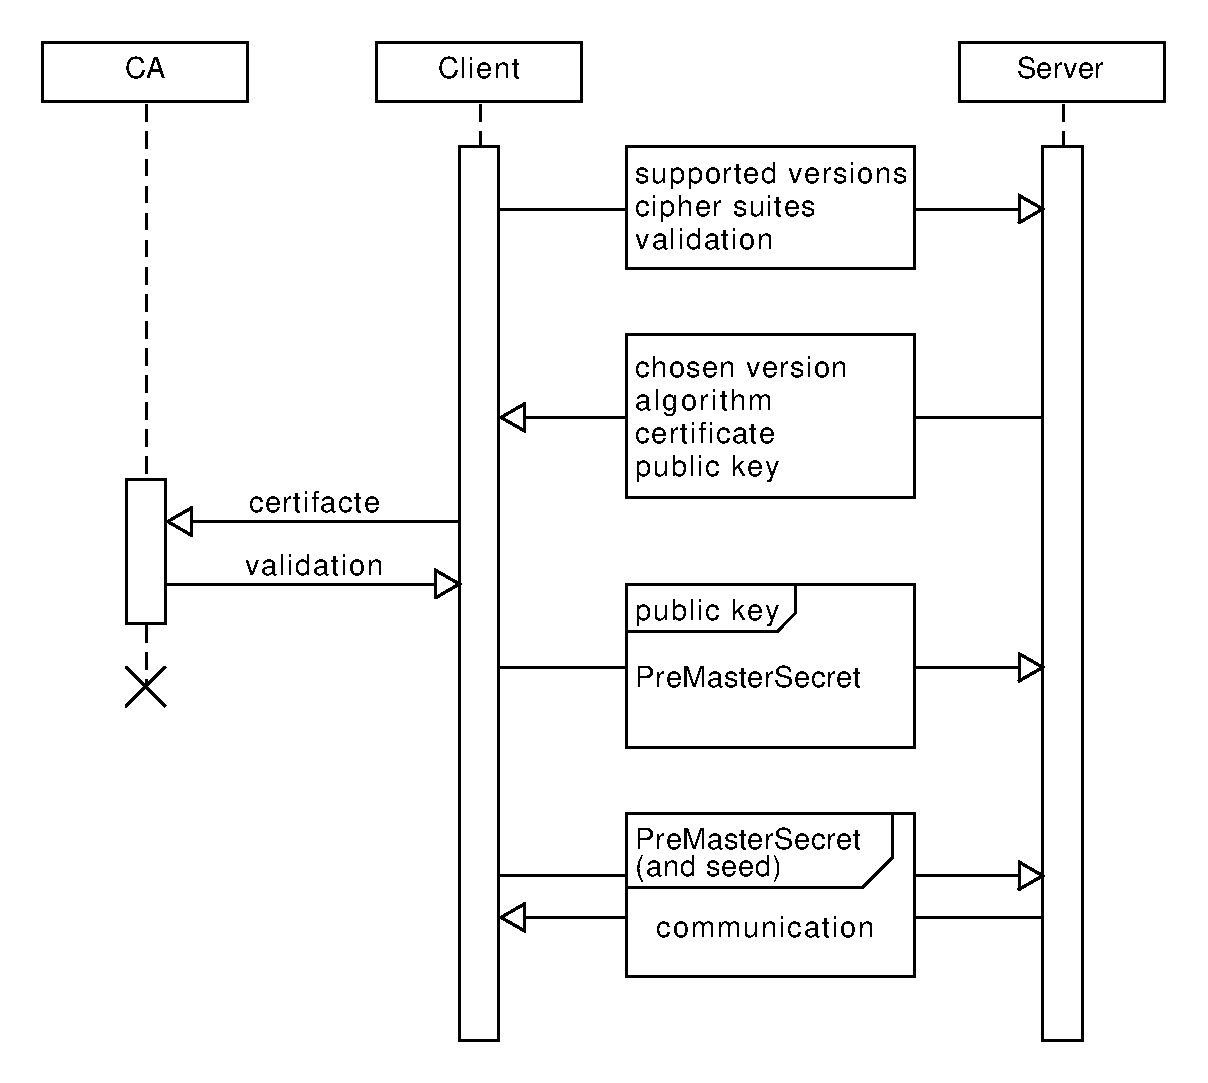
\includegraphics[width=0.7\textwidth]{security/tls.pdf}
    \caption{TLS handshake}
    \label{fig:tls}
\end{figure}
\FloatBarrier

For our purposes we have chosen to use what is called a self-signed certificate, because it covered the need for encryption that we had, and the price of a certificate issued by a CA is fairly high. The certificate we use was created by using OpenSSL\footnote{https://www.openssl.org}, which is an open source project that allows you to create your own certificate. One of the issues in utilizing a self-signed certificate is that the certificate will not be trusted by most browsers and operating systems. A more severe problem is the fact that it leaves the connection vulnerable to a man in the middle attack, where a third party with malicious intent might intercept the connection and use his own ``fake'' certificate and thereby getting access to potentially sensitive information. This would not be a problem if we had used a certificate issued by a CA, because the certificate then could be validated. Having a self-signed certificate also means that most browsers will not trust the certificate, and make the user of the browser aware that the site they are trying to connect to might be insecure with a scary warning page. 
Another problem is that the self-signed certificates are not trusted by Android, which causes problems when trying to make a connection to our server. To solve this problem Android provides the possibility of overriding what they call their \mono{TrustManager}, which we have done. 

\todo[inline]{insert snippet of trust manager override, and explain it above}

Another problem that we encountered with the Android platform is that there are issues when a certificate uses what is called wildcard subdomains. Wildcard subdomains allows us to use the same certificate for various server names mentioned in \secref{sub:server_names}. Therefore we used the wildcard domain ``\mono{*.*.ourdomain.dk}'' on our certificate. However, in case of wildcard subdomains the standard Android hostname verifier will try to check if the domain is an exact match to the requested hostname, which will fail and raise an exception. Luckily, the framework allows us to override their \mono{HostnameVerifier} as seen in \todo{insert hostname verifier ref}

\todo[inline]{Insert snippet of hostname verifier and describe it below}

Having the server placed on the university\todo{Det er første gang vi nævner at serveren er på Uni, det bliver beskrevet i reflection kapitlet (\secref{sec:the_android_platform_compatibility_and_test_driven_development}), det er måske ikke så godt?} did also introduce other problems, due to a limitation in what ports that we could use for outside access. 
We were assigned two different ports from outside access namely port 8000 and 8001, which we used for the web application, and our continious integration system respectively. 
If we had access to the ports normally used for the HTTP and HTTPS protocols, we could have used a system called let's encrypt \footnote{https://letsencrypt.org}, which is an free certificate authority trusted by all major browsers \parencite{lets_encrypt_all_browsers}. Let's encrypt allows for automatic verification of domain name ownership by installing their client on the server, where it will use port 80 and 443 to access validate a servers authenticity and create a certificate that can be validated through them. Using let's encrypt as our CA would remove the intimidating error potential customers encounter when accessing our page through most web browser, and also remove the need for overriding the \mono{HostnameVerifier} and the \mono{TrustManager} in the Android client code.